\chapter{Experiments and results} \label{sec:experiments-and-results}
Results trying to define a good baseline:


\section{Defining a baseline}
In order to do multiple experiments I needed a baseline to compare subsequent experiments with. There aren't any baselines on NeRFs with data gathered from CARLA, so I made my own. The baseline is put together by combining the best setup from the following categories:

CARLA:
\begin{itemize}
    \item Camera-setup
    \item Capacity
    \item Camera settings (image size)
    \item Vehicle speed
    \item Number of frames
\end{itemize}

NeRF:
\begin{itemize}
    \item Model
    \item Camera optimization
\end{itemize}













\subsection{Camera setup} \label{sec:exp-camera-setup}
The CARLA simulator provides a convenient way to attach multiple cameras with varying settings to a vehicle. To optimize the performance of NeRFs on RGB images, a series of experiments were conducted to determine the optimal camera setup based on the three metrics: PSNR, SSIM, LPIPS. All cameras were positioned at the same base translation, at the roof of the ego vehicle approximately 3 meters above ground level. While this camera placement may be considered unrealistically elevated, it facilitates an unobstructed capture of the scene without interference from the ego vehicle. The camera setups tested in this study were:

% TODO: Add figure with the camera setups?
\begin{itemize}
    \item Single forward-facing camera.
    \item Two forward-facing cameras, with a counterrotated yaw.
    \item Three cameras, one with zero yaw and two with counterrotated yaw.
\end{itemize}

\begin{table}[ht]
\centering
\setlength{\tabcolsep}{12pt}
\renewcommand{\arraystretch}{1.2}
\begin{tabular}{l l}
\multicolumn{2}{c}{\textbf{Experiment setup - constant variables}} \\
\hline
Parameter & Value \\
\hline
Distance  & 125 meters \\
Image resolution &  $600 \times 450$ \\
Ticks per image & 3 \\
Speed & 100\% (default: 30km/h) \\
\hline
\end{tabular}
\caption{Overview of the values of the parameters that remained constant across the runs in the experiment.}
\label{tab:camera-setup-stable-variables}
\end{table}


\begin{table}[ht]
\centering
\setlength{\tabcolsep}{6pt}
\renewcommand{\arraystretch}{1.5}
\begin{tabular}{l l | C{2.2} C{1.3} C{1.3}}
\hline
& \textbf{Description} & \textbf{PSNR $\uparrow$} & \textbf{SSIM $\uparrow$} & \textbf{LPIPS $\downarrow$} \\
\hline
0 & Single camera, $[0^{\circ}]$ yaw & 22.764567 & 0.74230 & 0.150325 \\
\cellcolor{blue}0 &\cellcolor{blue}Two cameras, $[-10^{\circ}, 10^{\circ}]$ yaw & 23.900909 & \cellcolor{green} 0.782013 & \cellcolor{green} 0.135604 \\
1 & Two cameras, $[-30^{\circ}, 30^{\circ}]$ yaw & \cellcolor{red} 23.235004 & 0.755689 & 0.155470 \\
2 & Two cameras, $[-50^{\circ}, 50^{\circ}]$ yaw & 23.732924 & \cellcolor{red} 0.739246 & 0.174111 \\
3 & Two cameras, $[-70^{\circ}, 70^{\circ}]$ yaw & \cellcolor{green} 24.318214 & 0.739551 & 0.172868 \\
4 & Three cameras,  $[-50^{\circ}, 0^{\circ}, 50^{\circ}]$ yaw & 23.785522 & 0.763684 & 0.165152 \\
5 & Three cameras,  $[-70^{\circ}, 0^{\circ}, 70^{\circ}]$ yaw & 23.684502 & 0.754842 & \cellcolor{red} 0.176524 \\
\hline
\end{tabular}
\caption{Comparison of camera setups for experiment \texttt{exp\_camera\_setup-5}. The table shows the results for different camera setups, where \ulcolor[blue]{blue} indicates the setup chosen for further experiments, \ulcolor[green]{green} indicates the best results, and \ulcolor[red]{red} indicates the worst results.}
\label{tab:exp_camera_setup-5}
\end{table}


% Overall, the results suggest that a camera setup with two cameras at -10$^{\circ}$ and 10$^{\circ}$ yaw produces the highest quality images, while setups with more than two cameras do not necessarily result in significantly higher quality images
From the table, we can see that the camera setups produce relatively similar results across the three metrics, with only small differences between them. The camera setup with two cameras at -70$^{\circ}$ and 70$^{\circ}$ yaw (Setup 3) achieves the highest PSNR score, indicating that it produces the most accurate images. On the other hand, camera setup 1 with two cameras at $-10^{\circ}$ and $10^{\circ}$ yaw achieves the highest SSIM and lowest LPIPS scores, indicating that it produces the most visually similar and perceptually pleasing images. Due to setup 0's high SSIM and low LPIPS, it was chosen as the camera setup baseline for further experiments.

% ADD THIS TO THE DISCUSSION-PART
% The reason for -10 and 10 being the best performing: Trained more on the images it was later evaluated on, since the evaluation images are 10% of the original training data.



























\subsection{Capacity} \label{sec:exp-capacity}
As discussed in \autoref{sec:large-scale-nerf} and \autoref{sec:method-block-nerf}, the capacity of a NeRF is limited. In order to quantitatively assess this capacity, we designed an experiment involving five increasingly longer routes for a CARLA vehicle to gather data on, ranging from 50m to approximately 450m in length, as depicted in Figure \ref{fig:capacity-overview}. The longest route corresponds to a full lap around the block. The collected data was then utilized in the NeRF pipeline for training, evaluation, and rendering of a resulting NeRF.

\begin{table}[ht]
\centering
\setlength{\tabcolsep}{12pt}
\renewcommand{\arraystretch}{1.2}
\begin{tabular}{l l}
\multicolumn{2}{c}{\textbf{Experiment setup - constant variables}} \\
\hline
Parameter & Value \\
\hline
\cellcolor{blue}Camera setup &\cellcolor{blue}Baseline from \autoref{sec:exp-camera-setup} \\
Image resolution &  $600 \times 450$ \\
Ticks per image & 3 \\
Speed & 100\% (default: 30km/h) \\
\hline
\end{tabular}
\caption{Overview of the values of the parameters that remained constant across the runs in the experiment.}
\label{tab:exp-capacity-stable-variables}
\end{table}

\begin{table}[ht]
\centering
\setlength{\tabcolsep}{6pt}
\renewcommand{\arraystretch}{1.5}
\begin{tabular}{l l | C{2.2} C{1.3} C{1.3}}
\hline
& \textbf{Description} & \textbf{PSNR $\uparrow$} & \textbf{SSIM $\uparrow$} & \textbf{LPIPS $\downarrow$} \\
\hline
0 & 50 meters & 23.541059 & \cellcolor{green} 0.773228 & \cellcolor{green} 0.108571 \\
1 & 100 meters & 23.594120 & 0.763471 & 0.141350 \\
2 & 2 turns & \cellcolor{green} 23.599499 & 0.756889 & 0.181586 \\
3 & 3 turns & 22.634428 & 0.719888 & 0.210503 \\
\cellcolor{blue}4 &\cellcolor{blue}4 turns & \cellcolor{red} 22.500532 & \cellcolor{red} 0.695553 & \cellcolor{red} 0.240513 \\
\hline
\end{tabular}
\caption{Comparison of NeRF's capacity for experiment \texttt{exp\_capacity-2}. The table shows the results for different distances and number of turns in the driving trajectory, where \ulcolor[blue]{blue} indicates the configuration chosen for further experiments, \ulcolor[green]{green} indicates the best results, and \ulcolor[red]{red} indicates the worst results.}
\label{tab:exp_capacity-2}
\end{table}



\begin{figure}[!h]
    \centering
    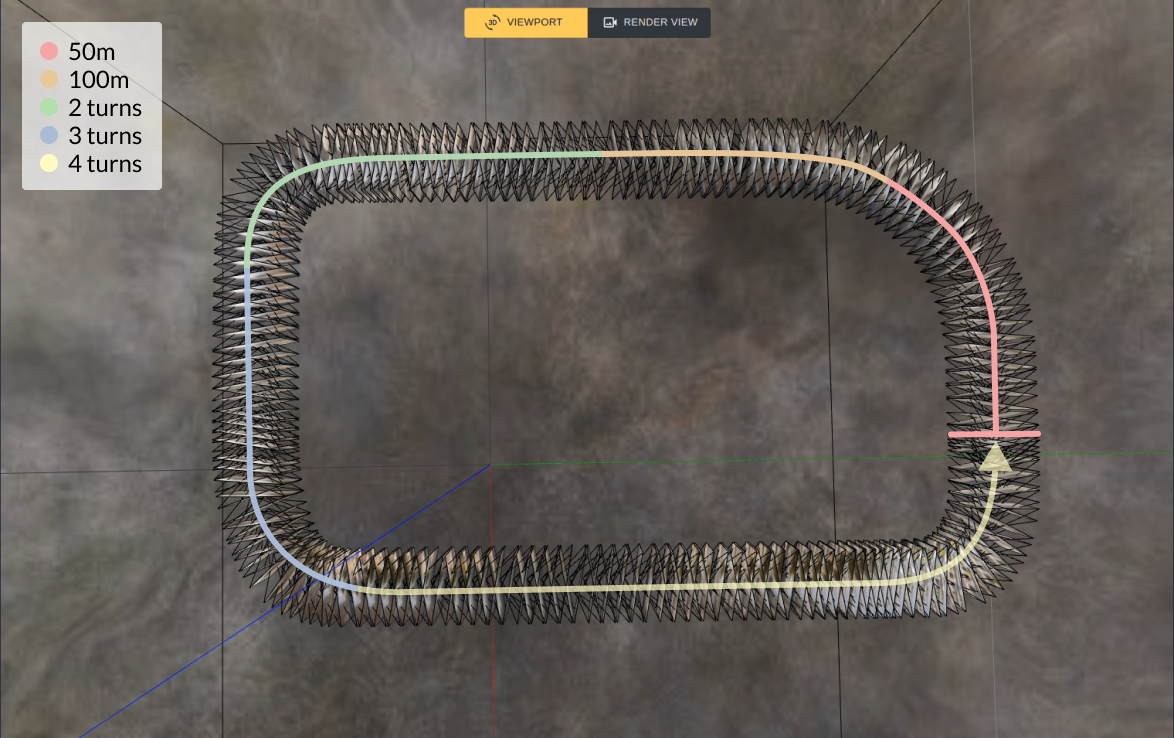
\includegraphics[width=1.0\textwidth]{figures/capacity-overview.png}
    \caption[Overview of the segments used in Experiment 1.2.]{Overview of the increasingly longer routes used to capture data in CARLA, during experiment 1.2.}
    \label{fig:capacity-overview}
\end{figure}

% ADD THIS TO THE DISCUSSION-PART
As expected, the results show that the quality of the rendered images degrades as the segments’ length increases. The PSNR remains relatively constant across the segments, while the SSIM and LPIPS metrics show a clear downward trend. The longest segment, the full lap around the block which includes four turns, results in the lowest quality images. Despite achieving the worst results, we selected the longest run as the baseline for further experiments. This is because conducting experiments on a full lap around the block provides a more realistic scenario for evaluating the performance of the NeRF on data captured by a vehicle. The full lap encompasses a variety of different scenes, including straight roads, curves, intersections, and varying lighting conditions. This diverse range of environments can help to test the NeRF’s ability to learn a varying scene and provide a more comprehensive evaluation of its performance.

























%The default number of frames to train on in Nerfstudio is 300, as written in their documentation. As seen in PROSJEKTOPPGAVEN, the quality of the trained NeRF should be better when trained on a larger dataset of images.

\subsection{Number of frames} \label{sec:exp-number-of-frames}
The number of input images used to train the NeRF should significantly affect its performance. The amount of images determines the amount of information available for the NeRF to learn the underlying 3D scene structure and appearance. A larger number of input images can provide more diverse and detailed information about the scene, which can help the NeRF to capture fine-grained details and generalize better to novel views. Given that the NeRF is set to sample batches across all input images, as is the case in our configuration and discussed in \autoref{sec:nerfstudio-pipeline}, a larger set of input images should result in higher-quality image synthesis. To test this hypothesis, we conducted an experiment in which we varied the number of frames grabbed from a CARLA run, resulting in different-sized datasets. The results of this experiment are shown in \autoref{tab:exp_frames-2}.

\begin{table}[ht]
\centering
\setlength{\tabcolsep}{12pt}
\renewcommand{\arraystretch}{1.2}
\begin{tabular}{l l}
\multicolumn{2}{c}{\textbf{Experiment setup - constant variables}} \\
\hline
Parameter & Value \\
\hline
\cellcolor{blue}Camera setup &\cellcolor{blue}Baseline from \autoref{sec:exp-camera-setup} \\
\cellcolor{blue}Distance &\cellcolor{blue}Baseline from \autoref{sec:exp-capacity} \\
Image resolution &  $600 \times 450$ \\
Speed & 100\% (default: 30km/h) \\
\hline
\end{tabular}
\caption{Overview of the values of the parameters that remained constant across the runs in the experiment.}
\label{tab:exp-number-of-frames-stable-variables}
\end{table}

\begin{table}[ht]
\centering
\setlength{\tabcolsep}{6pt}
\renewcommand{\arraystretch}{1.5}
\begin{tabular}{l l | C{2.2} C{1.3} C{1.3}}
\hline
& \textbf{Description} & \textbf{PSNR $\uparrow$} & \textbf{SSIM $\uparrow$} & \textbf{LPIPS $\downarrow$} \\
\hline
0 & Image every tick & \cellcolor{green} 23.258400 & 0.723872 & 0.228383 \\
\cellcolor{blue}1 &\cellcolor{blue}Image every 2$^{\text{nd}}$ tick & 23.251682 & \cellcolor{green} 0.727191 & \cellcolor{green} 0.221351 \\
2 & Image every 3$^{\text{rd}}$ tick & 22.557207 & 0.696930 & 0.239964 \\
3 & Image every 4$^{\text{th}}$ tick & 22.219042 & 0.685168 & 0.250390 \\
4 & Image every 5$^{\text{th}}$ tick & \cellcolor{red} 21.917959 & \cellcolor{red} 0.678348 & \cellcolor{red} 0.258932 \\
\hline
\end{tabular}
\caption{Comparison of image capture frequency for experiment \texttt{exp\_frames-2}. The table shows the results for different image capture frequencies, where \ulcolor[blue]{blue} indicates the configuration chosen for further experiments, \ulcolor[green]{green} indicates the best results, and \ulcolor[red]{red} indicates the worst results.}
\label{tab:exp_frames-2}
\end{table}

As we can see from the table, the trained NeRF performs better on the metrics when trained on a larger dataset of images. There is almost no difference between grabbing an image every frame and grabbing an image every second frame. Therefore, we selected the latter option, grabbing an image every second frame, for further experiments due to the performance of the CARLA- and NeRF-pipeline.

























\subsection{Image size} \label{sec:exp-image-resolution}
CARLA allows users to define the image resolution outputted by mounted cameras. In order to test to what degree the input image resolution has on the output image synthesis, I captured data from CARLA at 5 increasingly higher image resolutions. The results can be seen in \autoref{tab:exp_image_size-2}

\begin{table}[ht]
\centering
\setlength{\tabcolsep}{12pt}
\renewcommand{\arraystretch}{1.2}
\begin{tabular}{l l}
\multicolumn{2}{c}{\textbf{Experiment setup - constant variables}} \\
\hline
Parameter & Value \\
\hline
\cellcolor{blue}Camera setup &\cellcolor{blue}Baseline from \autoref{sec:exp-camera-setup} \\
\cellcolor{blue}Distance &\cellcolor{blue}Baseline from \autoref{sec:exp-capacity} \\
\cellcolor{blue}Ticks per image &\cellcolor{blue}Baseline from \autoref{sec:exp-number-of-frames} \\
Speed & 100\% (default: 30km/h) \\
\hline
\end{tabular}
\caption{Overview of the values of the parameters that remained constant across the runs in the experiment.}
\label{tab:exp-image-resolution-stable-variables}
\end{table}

\begin{table}[ht]
\centering
\setlength{\tabcolsep}{6pt}
\renewcommand{\arraystretch}{1.5}
\begin{tabular}{l l | C{2.2} C{1.3} C{1.3}}
\hline
& \textbf{Description} & \textbf{PSNR $\uparrow$} & \textbf{SSIM $\uparrow$} & \textbf{LPIPS $\downarrow$} \\
\hline
0 & Image resolution of $200 \times 150$ & 23.349852 & 0.748548 & \cellcolor{green} 0.081860 \\
\cellcolor{blue}1 &\cellcolor{blue}Image resolution of $400 \times 300$ & \cellcolor{green} 23.613869 & \cellcolor{green} 0.775704 & 0.103645 \\
2 & Image resolution of $800 \times 600$ & 23.242430 & 0.762787 & 0.168621 \\
3 & Image resolution of $1200 \times 900$ & 23.073208 & 0.731756 & 0.232993 \\
4 & Image resolution of $1600 \times 1200$ & \cellcolor{red} 22.822489 & \cellcolor{red} 0.727354 & \cellcolor{red} 0.267016 \\
\hline
\end{tabular}
\caption{Comparison of image resolution for experiment \texttt{exp\_image\_size-2}. The table shows the results for different image resolutions, where \ulcolor[blue]{blue} indicates the configuration chosen for further experiments, \ulcolor[green]{green} indicates the best results, and \ulcolor[red]{red} indicates the worst results.}
\label{tab:exp_image_size-2}
\end{table}

This experiment provides a clear example of how important it is to also consider the visual quality of the image synthesis and not only rely on the reported metrics. \autoref{fig:image-size-comparison} depicts the resulting image synthesis of the same frame across the model trained on low-res, medium-res, and high-res data. Although the reported metrics indicate that the $200 /times 150$-dataset performs best, the rendered frame clearly shows that the NeRF trained on higher-resolution data is able to represent fine-grained details and produce more visually pleasing images. Based on both the qualitative and quantitative assessments, setup 1 was chosen as the baseline for further experiments.

\begin{figure}[h]
    \centering
    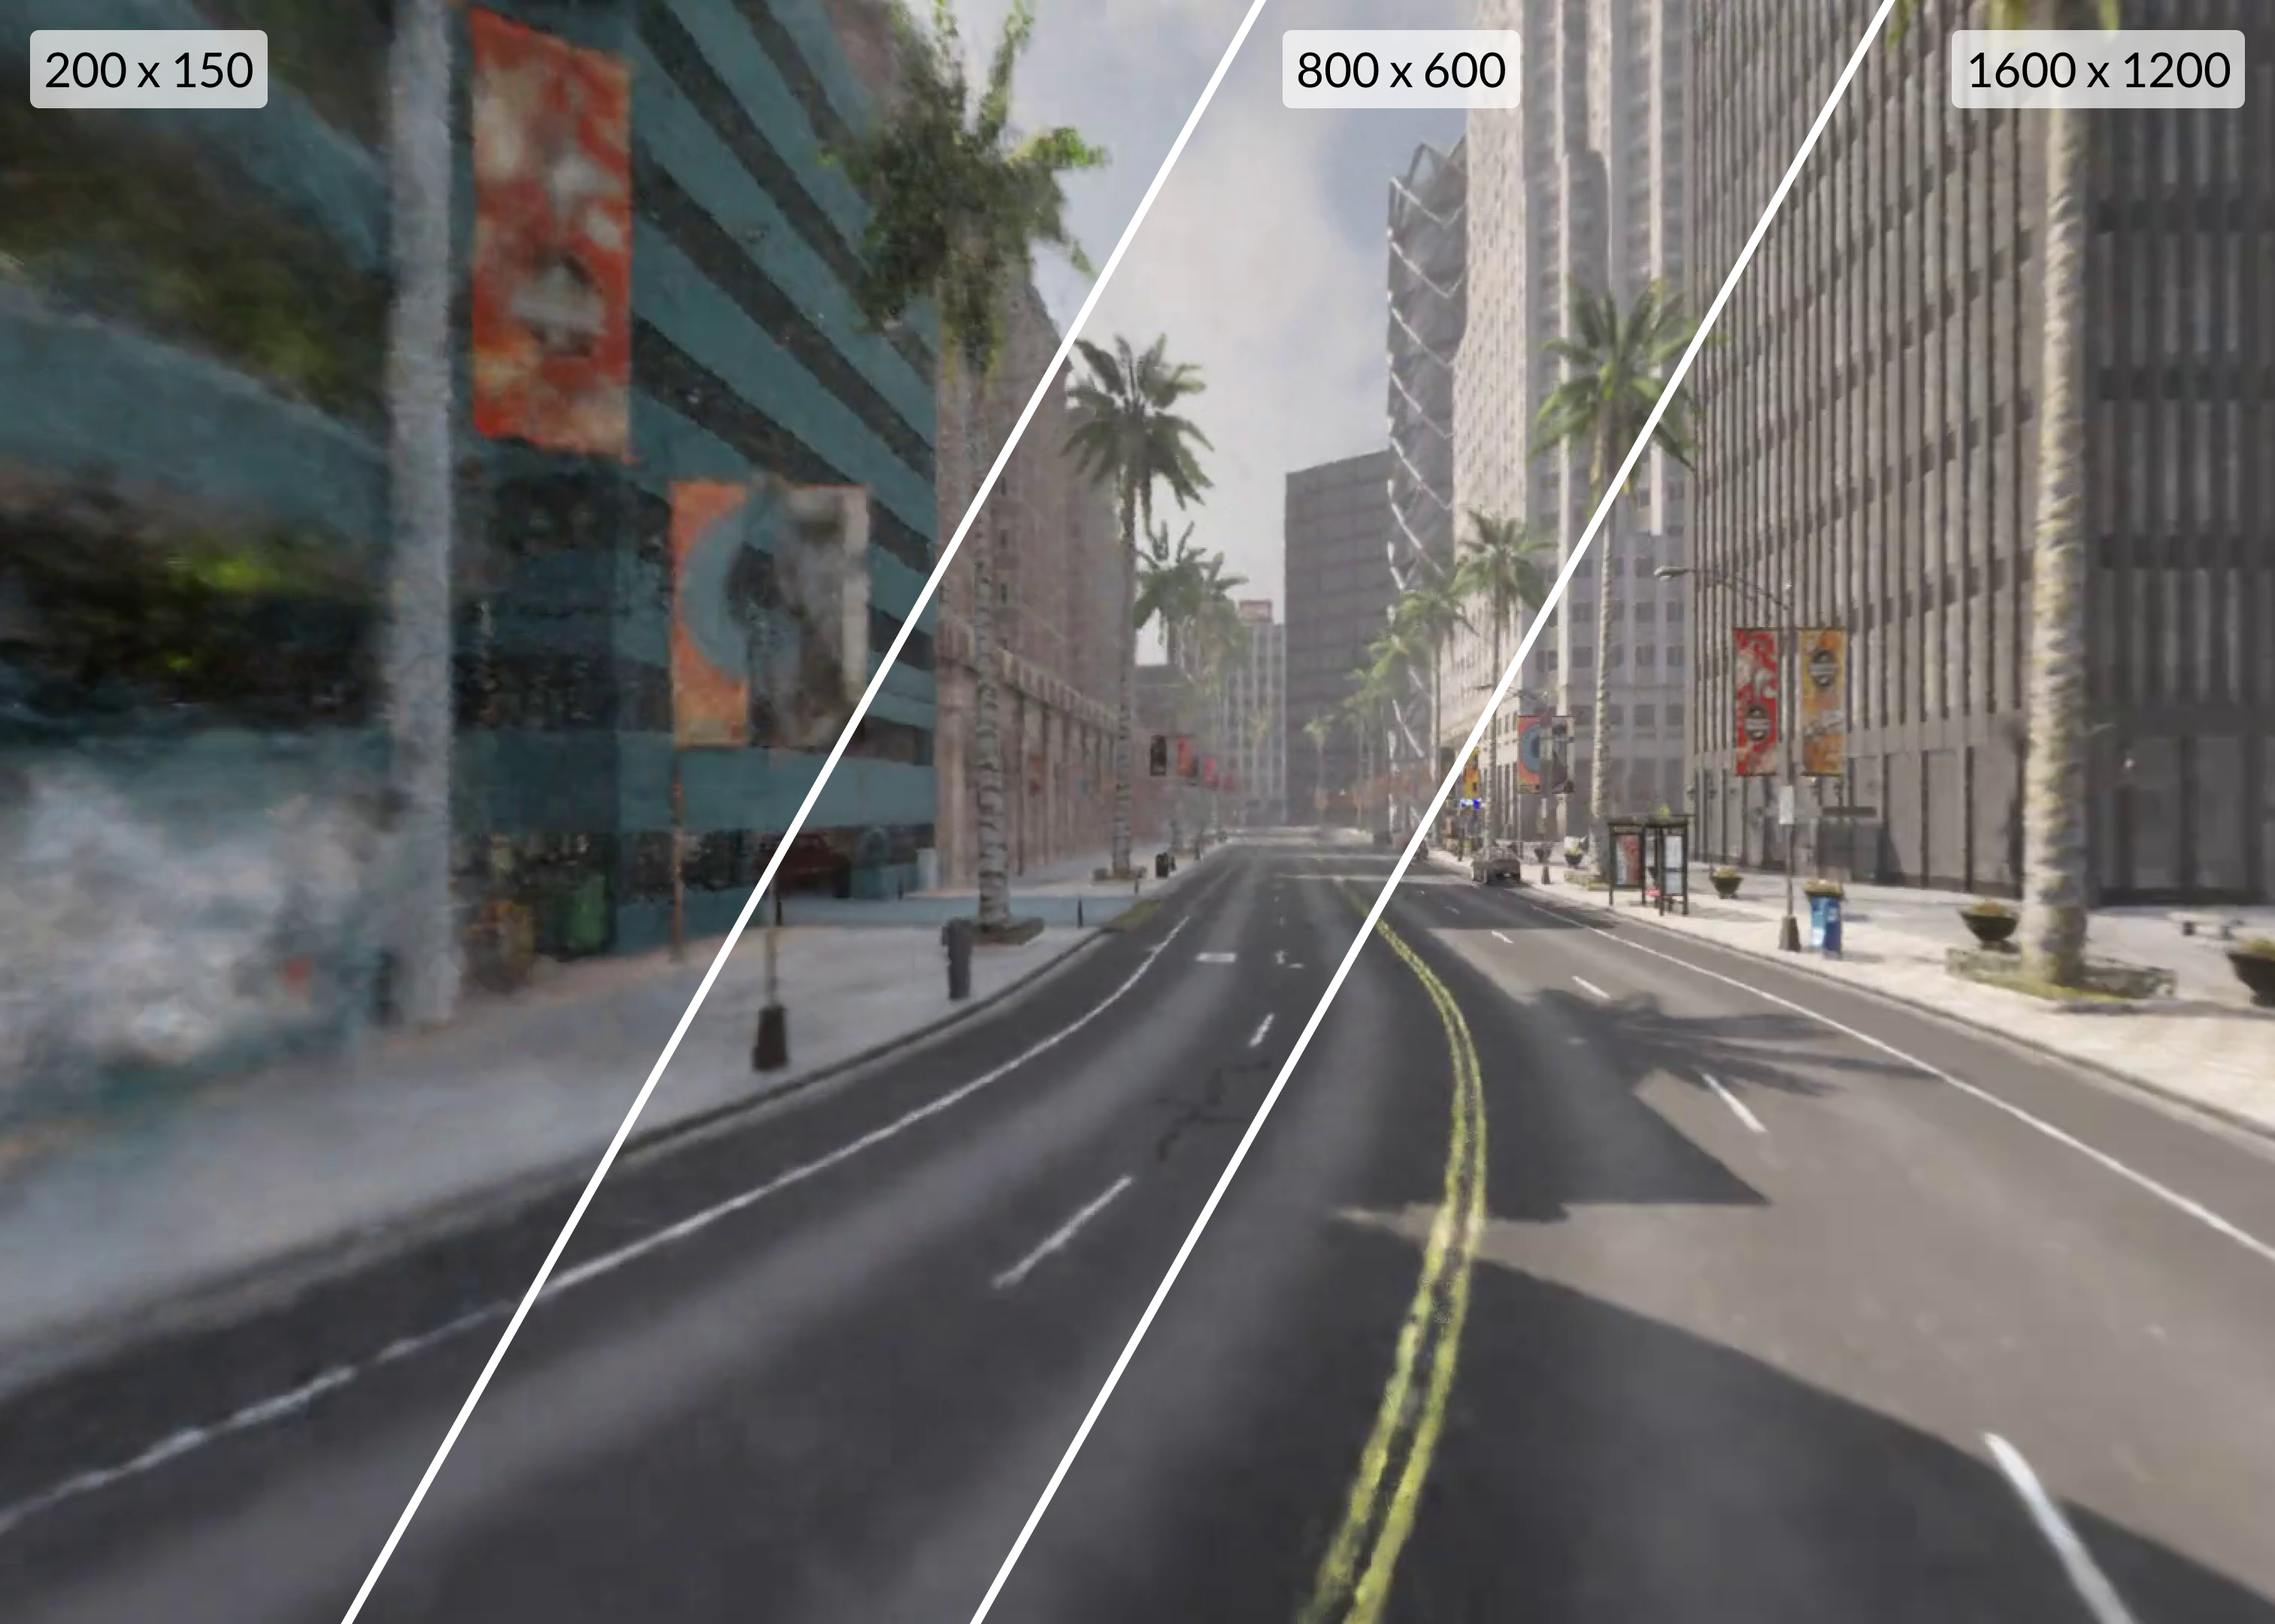
\includegraphics[width=1.0\textwidth]{figures/image-size-comparison.png}
    \caption{Comparison of frames rendered from models trained with training-data of different image resolution.}
    \label{fig:image-size-comparison}
\end{figure}

% Add to discussion
% When using lower resolution images, the LPIPS and SSIM metrics may become less sensitive because they are less affected by small differences between the synthesized and ground-truth images. This is because lower resolution images have fewer pixels, which can make the metrics less precise in measuring the perceptual similarity between the images. However, using lower resolution images can also lead to a loss of detail and fidelity in the synthesized images. When using high-resolution images, these metrics may become less effective because they are more sensitive to small differences between the synthesized and ground-truth images. In other words, the NeRF may generate high-quality images that are perceptually similar to the ground-truth images, but small differences in the pixel values or noise can cause a significant decrease in the LPIPS and SSIM scores.
% Why is there such a large difference in the LPIPS score, in contrary to the other metrics.



















\subsection{Vehicle speed} \label{sec:exp-speed}
The speed of the vehicle can affect the quality of the data captured by the mounted cameras in the CARLA simulator. To investigate the impact of vehicle speed on the quality of the data, we conducted a series of experiments at different speeds.


In order to test how much the vehicle speed contributes to the quality of data capture I performed 4 different experiments on vehicle speed.

\begin{table}[ht]
\centering
\setlength{\tabcolsep}{12pt}
\renewcommand{\arraystretch}{1.2}
\begin{tabular}{l l}
\multicolumn{2}{c}{\textbf{Experiment setup - constant variables}} \\
\hline
Parameter & Value \\
\hline
\cellcolor{blue}Camera setup &\cellcolor{blue}Baseline from \autoref{sec:exp-camera-setup} \\
\cellcolor{blue}Distance &\cellcolor{blue}Baseline from \autoref{sec:exp-capacity} \\
\cellcolor{blue}Ticks per image &\cellcolor{blue}Baseline from \autoref{sec:exp-number-of-frames} \\
\cellcolor{blue}Image resolution &\cellcolor{blue}Baseline from \autoref{sec:exp-image-resolution} \\
\hline
\end{tabular}
\caption{Overview of the values of the parameters that remained constant across the runs in the experiment.}
\label{tab:exp-speed-stable-variables}
\end{table}


\begin{table}[ht]
\centering
\setlength{\tabcolsep}{6pt}
\renewcommand{\arraystretch}{1.5}
\begin{tabular}{l l | C{2.2} C{1.3} C{1.3}}
\hline
& \textbf{Description} & \textbf{PSNR $\uparrow$} & \textbf{SSIM $\uparrow$} & \textbf{LPIPS $\downarrow$} \\
\hline
\cellcolor{blue}0 &\cellcolor{blue}50\% speed & \cellcolor{green} 24.061440 & \cellcolor{green} 0.775393 & \cellcolor{green} 0.181360 \\
1 & 100\% speed & 23.502066 & 0.755476 & 0.184455 \\
2 & 150\% speed & 23.411259 & 0.742473 & 0.189968 \\
3 & 200\% speed & \cellcolor{red} 22.717318 & \cellcolor{red} 0.713858 & \cellcolor{red} 0.200099 \\
\hline
\end{tabular}
\caption{Comparison of vehicle speed for experiment \texttt{exp\_speed-2}. The table shows the results for different vehicle speeds, where \ulcolor[blue]{blue} indicates the configuration chosen for further experiments, \ulcolor[green]{green} indicates the best results, and \ulcolor[red]{red} indicates the worst results.}
\label{tab:exp_speed-2}
\end{table}

The results of our experiments, shown in \autoref{tab:exp_speed-2}, indicate that the speed of the vehicle has a significant impact on the quality of the data captured by the mounted cameras. Specifically, we observe that the NeRF trained on the data captured at 50\% speed achieves the highest scores on all three metrics (PSNR, SSIM, and LPIPS), while the NeRF trained on the data captured at 200\% speed achieves the lowest scores on all three metrics. This suggests that slower vehicle speeds can lead to higher-quality data capture, while faster vehicle speeds can lead to lower-quality data capture. The reason for this can be attributed to the motion blur and temporal artifacts that can occur when the vehicle is moving too fast. At higher speeds, the motion of the vehicle can cause blurring and distortion in the captured images, which can reduce the quality of the data and make it more difficult for the NeRF to learn the underlying 3D scene structure and appearance. In contrast, slower vehicle speeds can reduce the amount of motion blur and temporal artifacts, resulting in clearer and more detailed images. Another side effect of driving slower is that it leads to increased amount of images captured. At 50\% speed, the dataset consists of 351 images, in contrast to the 131 images captured at 200\% speed.














































\subsection{Combined baseline}
The combined baseline in our experiments is the configuration that yielded the best results across all the experiments, with the exception of the baseline's drive distance. It consists of two forward-facing RGB-cameras, counterrotated with $-10^\circ$- and $10^\circ$ yaw, capturing images every second tick, along a city-block that spans 450 meters in distance, with an image size of $400 \times 300$, and a vehicle speed that's 50\% slower than the default of 30 km/h. The results of our experiments shown in \autoref{tab:exp_combined_baseline_2-0} demonstrates that the combined baseline achieves high scores across all three metrics, PSNR, SSIM, and LPIPS, indicating that this configuration leads to a high-quality data capture and good performance of the NeRF. Due to this, the combined baseline can serve as a useful starting point for future research and applications.

\begin{table}[ht]
\centering
\setlength{\tabcolsep}{12pt}
\renewcommand{\arraystretch}{1.2}
\begin{tabular}{l l}
\multicolumn{2}{c}{\textbf{Experiment setup - constant variables}} \\
\hline
Parameter & Value \\
\hline
\cellcolor{blue}Camera setup &\cellcolor{blue}Baseline from \autoref{sec:exp-camera-setup} \\
\cellcolor{blue}Distance &\cellcolor{blue}Baseline from \autoref{sec:exp-capacity} \\
\cellcolor{blue}Ticks per image &\cellcolor{blue}Baseline from \autoref{sec:exp-number-of-frames} \\
\cellcolor{blue}Image resolution &\cellcolor{blue}Baseline from \autoref{sec:exp-image-resolution} \\
\cellcolor{blue}Speed &\cellcolor{blue}Baseline from \autoref{sec:exp-speed} \\
\hline
\end{tabular}
\caption{Overview of the values of the parameters that remained constant across the runs in the experiment.}
\label{tab:exp-combined-baseline-stable-variables}
\end{table}

\begin{table}[ht]
\centering
\setlength{\tabcolsep}{6pt}
\renewcommand{\arraystretch}{1.5}
\begin{tabular}{l l | C{2.2} C{1.3} C{1.3}}
\hline
& \textbf{Description} & \textbf{PSNR $\uparrow$} & \textbf{SSIM $\uparrow$} & \textbf{LPIPS $\downarrow$} \\
\hline
0 & Combined baseline & 24.197817 & 0.766733 & 0.168807 \\
\hline
\end{tabular}
\caption{Results for exp\_combined\_baseline\_2-0}
\label{tab:exp_combined_baseline_2-0}
\end{table}















\section{Adding noise}
Hypothesis: The camera optimization works better on short segments, which entails that Block-NeRF will have a even greater benefit when the scene is large.

\begin{comment}
Information about GNSS-error
https://junipersys.com/support/article/6614#:~:text=Just%20as%20a%20general%20observation,to%202%20m%20vertical%20accuracy.
\end{comment}

\begin{table}[ht]
\centering
\setlength{\tabcolsep}{6pt}
\renewcommand{\arraystretch}{1.5}
\begin{tabular}{l l | C{2.2} C{1.3} C{1.3}}
\hline
& \textbf{Description} & \textbf{PSNR $\uparrow$} & \textbf{SSIM $\uparrow$} & \textbf{LPIPS $\downarrow$} \\
\hline
\multicolumn{5}{c}{\textbf{Baseline \textbf{with} camera optimizer}} \\
\hline
0 & $\mathcal{N}(0, 0)$ & \cellcolor{green} 23.609739 & \cellcolor{green} 0.754924 & \cellcolor{green} 0.171715 \\
1 & $\mathcal{N}(0, 0.5^2)$ & 18.499672 & 0.486572 & 0.240731 \\
2 & $\mathcal{N}(0, 1^2)$ & 16.924616 & 0.407149 & 0.297813 \\
3 & $\mathcal{N}(0, 3^2)$ & \cellcolor{red} 16.297756 & \cellcolor{red} 0.384611 & \cellcolor{red} 0.553038 \\
\hline
\multicolumn{5}{c}{\textbf{Baseline \textbf{without} camera optimizer}} \\
\hline
0 & $\mathcal{N}(0, 0)$ & \cellcolor{green} 23.913687 & \cellcolor{green} 0.771429 & \cellcolor{green} 0.166504 \\
1 & $\mathcal{N}(0, 0.5^2)$ & 19.446724 & 0.503864 & 0.414767 \\
2 & $\mathcal{N}(0, 1^2)$ & 18.099987 & 0.438293 & 0.482692 \\
3 & $\mathcal{N}(0, 3^2)$ & \cellcolor{red} 15.964767 & \cellcolor{red} 0.381585 & \cellcolor{red} 0.590534 \\
\hline
\end{tabular}
\caption{Results for \texttt{exp\_gaussian\_noise-2} and \texttt{exp\_gaussian\_noise\_no\_optimizer-2}. The optimizer run with optimizer seems to secure better and more stable LPIPS.}
\label{tab:exp_gaussian_noise-2}
\end{table}

\begin{table}[ht]
\centering
\setlength{\tabcolsep}{6pt}
\renewcommand{\arraystretch}{1.5}
\begin{tabular}{l l | C{2.2} C{1.3} C{1.3}}
\hline
& \textbf{Description} & \textbf{PSNR $\uparrow$} & \textbf{SSIM $\uparrow$} & \textbf{LPIPS $\downarrow$} \\
\hline
0 & $\mathcal{N}(0, 0^2)$ & \cellcolor{green} 24.795582 & \cellcolor{green} 0.833400 & \cellcolor{green} 0.102616 \\
1 & $\mathcal{N}(0, 0.1^2)$ & 22.735580 & 0.725762 & 0.121869 \\
2 & $\mathcal{N}(0, 0.2^2)$ & 20.316860 & 0.597075 & 0.152559 \\
3 & $\mathcal{N}(0, 0.3^2)$ & \cellcolor{red} 19.765114 & \cellcolor{red} 0.550024 & \cellcolor{red} 0.172539 \\
\bottomrule
\end{tabular}
\caption{Results for exp\_gaussian\_noise\_shorter\_segments-2}
\label{tab:exp_gaussian_noise_shorter_segments-2}
\end{table}



As seen in \autoref{tab:exp_gaussian_noise_shorter_segments-2} the metrics show better results than \autoref{tab:exp_gaussian_noise-2}. The noise seems to have a greater impact on the resulting scene, the larger the scene is. 


















\section{COLMAP vs. Absolute poses}

The results are almost equal. Need to look at the qualitative results. I'm rerunning the experiment on IDUN.

\begin{comment}   
{
  "experiment_name": "exp_combined_baseline_2_colmap_REDONE-0",
  "method_name": "nerfacto",
  "checkpoint": "data/images/exp_combined_baseline_2_colmap_REDONE/0/exp_combined_baseline_2_colmap_REDONE-0/nerfacto/2023-05-15_142558/nerfstudio_models/step-000014999.ckpt",
  "results": {
    "psnr": 23.396726608276367,
    "ssim": 0.7092073559761047,
    "lpips": 0.32087942957878113,
    "num_rays_per_sec": 741178.5625,
    "fps": 6.176488876342773
  }
}
\end{comment}



\begin{table}[ht]
\centering
\setlength{\tabcolsep}{6pt}
\renewcommand{\arraystretch}{1.5}
\begin{tabular}{l | C{2.2} C{1.3} C{1.3} c}
\hline
\textbf{Description} & \textbf{PSNR $\uparrow$} & \textbf{SSIM $\uparrow$} & \textbf{LPIPS $\downarrow$} & \textbf{Time processing} \\
\hline
Poses from CARLA & \cellcolor{green} 24.197817 & \cellcolor{green} 0.766733 & \cellcolor{red} 0.168807 &\cellcolor{green}00:00:00 \\% exp\_combined\_baseline\_2-0
Poses from COLMAP & \cellcolor{red} 24.18618 & \cellcolor{red} 0.758549 & \cellcolor{green} 0.159935 &\cellcolor{red}01:12:15 \\% data-images-exp\_combined\_baseline\_2\_colmap
\hline
\end{tabular}
\caption{Results for experiments}
\label{tab:colmap-vs-poses}
\end{table}



















\section{Different models}
Nerfstudio have implemented multiple well-known NeRF-models. In this experiment I'd like to see if changing the models would have any impact on the output.

- Nerfacto
- Nerfacto-big
- Instant-ngp





















\section{Block NeRF}

The naive Block NeRF implementation allows for the captured scene to be split into arbitrary number of segments. In this experiment, we'd like to explore the impact of segmenting the scene on the overall quality of the generated results. In particular, we compare the performance of Block NeRF to that of a single NeRF trained on the entire scene.

\autoref{tab:exp_combined_baseline_block_nerf} shows the result of splitting the baseline-scene into 4 segments, while \autoref{tab:exp_block_nerf_long_path_2-block_10} shows the result of splitting a longer scene into 12 segments. The qualitative results of the 12-segment run can be seen in \autoref{fig:block-nerf-comparison}.

%By splitting the scene into smaller segments, the combined scene generates better results than when the entire scene is trained within a single NeRF. The average PSNR is 24.4746 - which is 0.2768 better than the entire scene in one. Block NeRF's high quality will sustain large scenes, where a single NeRF will start deteriorating as the scene size increases.

\begin{table}[ht]
\centering
\setlength{\tabcolsep}{6pt}
\renewcommand{\arraystretch}{1.5}
\begin{tabular}{l l | C{2.2} C{1.3} C{1.3}}
\hline
& \textbf{Description} & \textbf{PSNR $\uparrow$} & \textbf{SSIM $\uparrow$} & \textbf{LPIPS $\downarrow$} \\
\hline
0 & Segment 1 & 24.960262 & 0.815270 & 0.161623 \\
1 & Segment 2 & 25.660400 & 0.824085 & 0.164296 \\
2 & Segment 3 & 23.914209 & 0.755183 & 0.194245 \\
3 & Segment 4 & 23.363695 & 0.764547 & 0.216242 \\
\hline
\multicolumn{2}{l}{Average difference from one NeRF} &\cellcolor{green} 0.2768 &\cellcolor{green} 0.02277125 &  \cellcolor{red} -0.015 % Unsure if I'll include this
\end{tabular}
\caption{Results for each segment when the basline-segment spanning the entire block has been split into 4 Block-NeRFs.}
\label{tab:exp_combined_baseline_block_nerf}
\end{table}


\begin{table}[ht]
\centering
\setlength{\tabcolsep}{6pt}
\renewcommand{\arraystretch}{1.5}
\begin{tabular}{l l | C{2.2} C{1.3} C{1.3}}
\hline
& \textbf{Description} & \textbf{PSNR $\uparrow$} & \textbf{SSIM $\uparrow$} & \textbf{LPIPS $\downarrow$} \\
\hline
0 & Segment 1 & 25.047100 & 0.826931 & 0.138852 \\
1 & Segment 2 & \cellcolor{green} 25.703838 & 0.831167 & 0.156331 \\
2 & Segment 3 & 24.924395 & 0.830144 & 0.149870 \\
3 & Segment 4 & \cellcolor{red} 22.726223 & \cellcolor{red} 0.713277 & \cellcolor{red} 0.207025 \\
4 & Segment 5 & 25.468483 & 0.837942 & \cellcolor{green} 0.131815 \\
5 & Segment 6 & 25.670006 & \cellcolor{green} 0.841962 & 0.147232 \\
6 & Segment 7 & 25.661350 & 0.820813 & 0.163685 \\
7 & Segment 8 & 25.070913 & 0.777114 & 0.154277 \\
8 & Segment 9 & 24.803871 & 0.814633 & 0.154028 \\
9 & Segment 10 & 23.693977 & 0.753770 & 0.185557 \\
10& Segment 11 & 23.936722 & 0.757462 & 0.179283 \\
11& Segment 12 & 24.584238 & 0.807874 & 0.144022 \\
\hline
\multicolumn{2}{l}{Average metrics of 12 block NeRF} & \cellcolor{green} 24.774259 & \cellcolor{green} 0.801090 & \cellcolor{green} 0.159331 \\
\multicolumn{2}{l}{Average metrics of 1 block NeRF} & \cellcolor{red} 22.515461 & \cellcolor{red} 0.654036 & \cellcolor{red} 0.424356 \\
\hline
\end{tabular}
\caption{Results for exp\_block\_nerf\_long\_path\_2-block\_10}
\label{tab:exp_block_nerf_long_path_2-block_10}
\end{table}

\begin{figure}[!h]
    \centering
    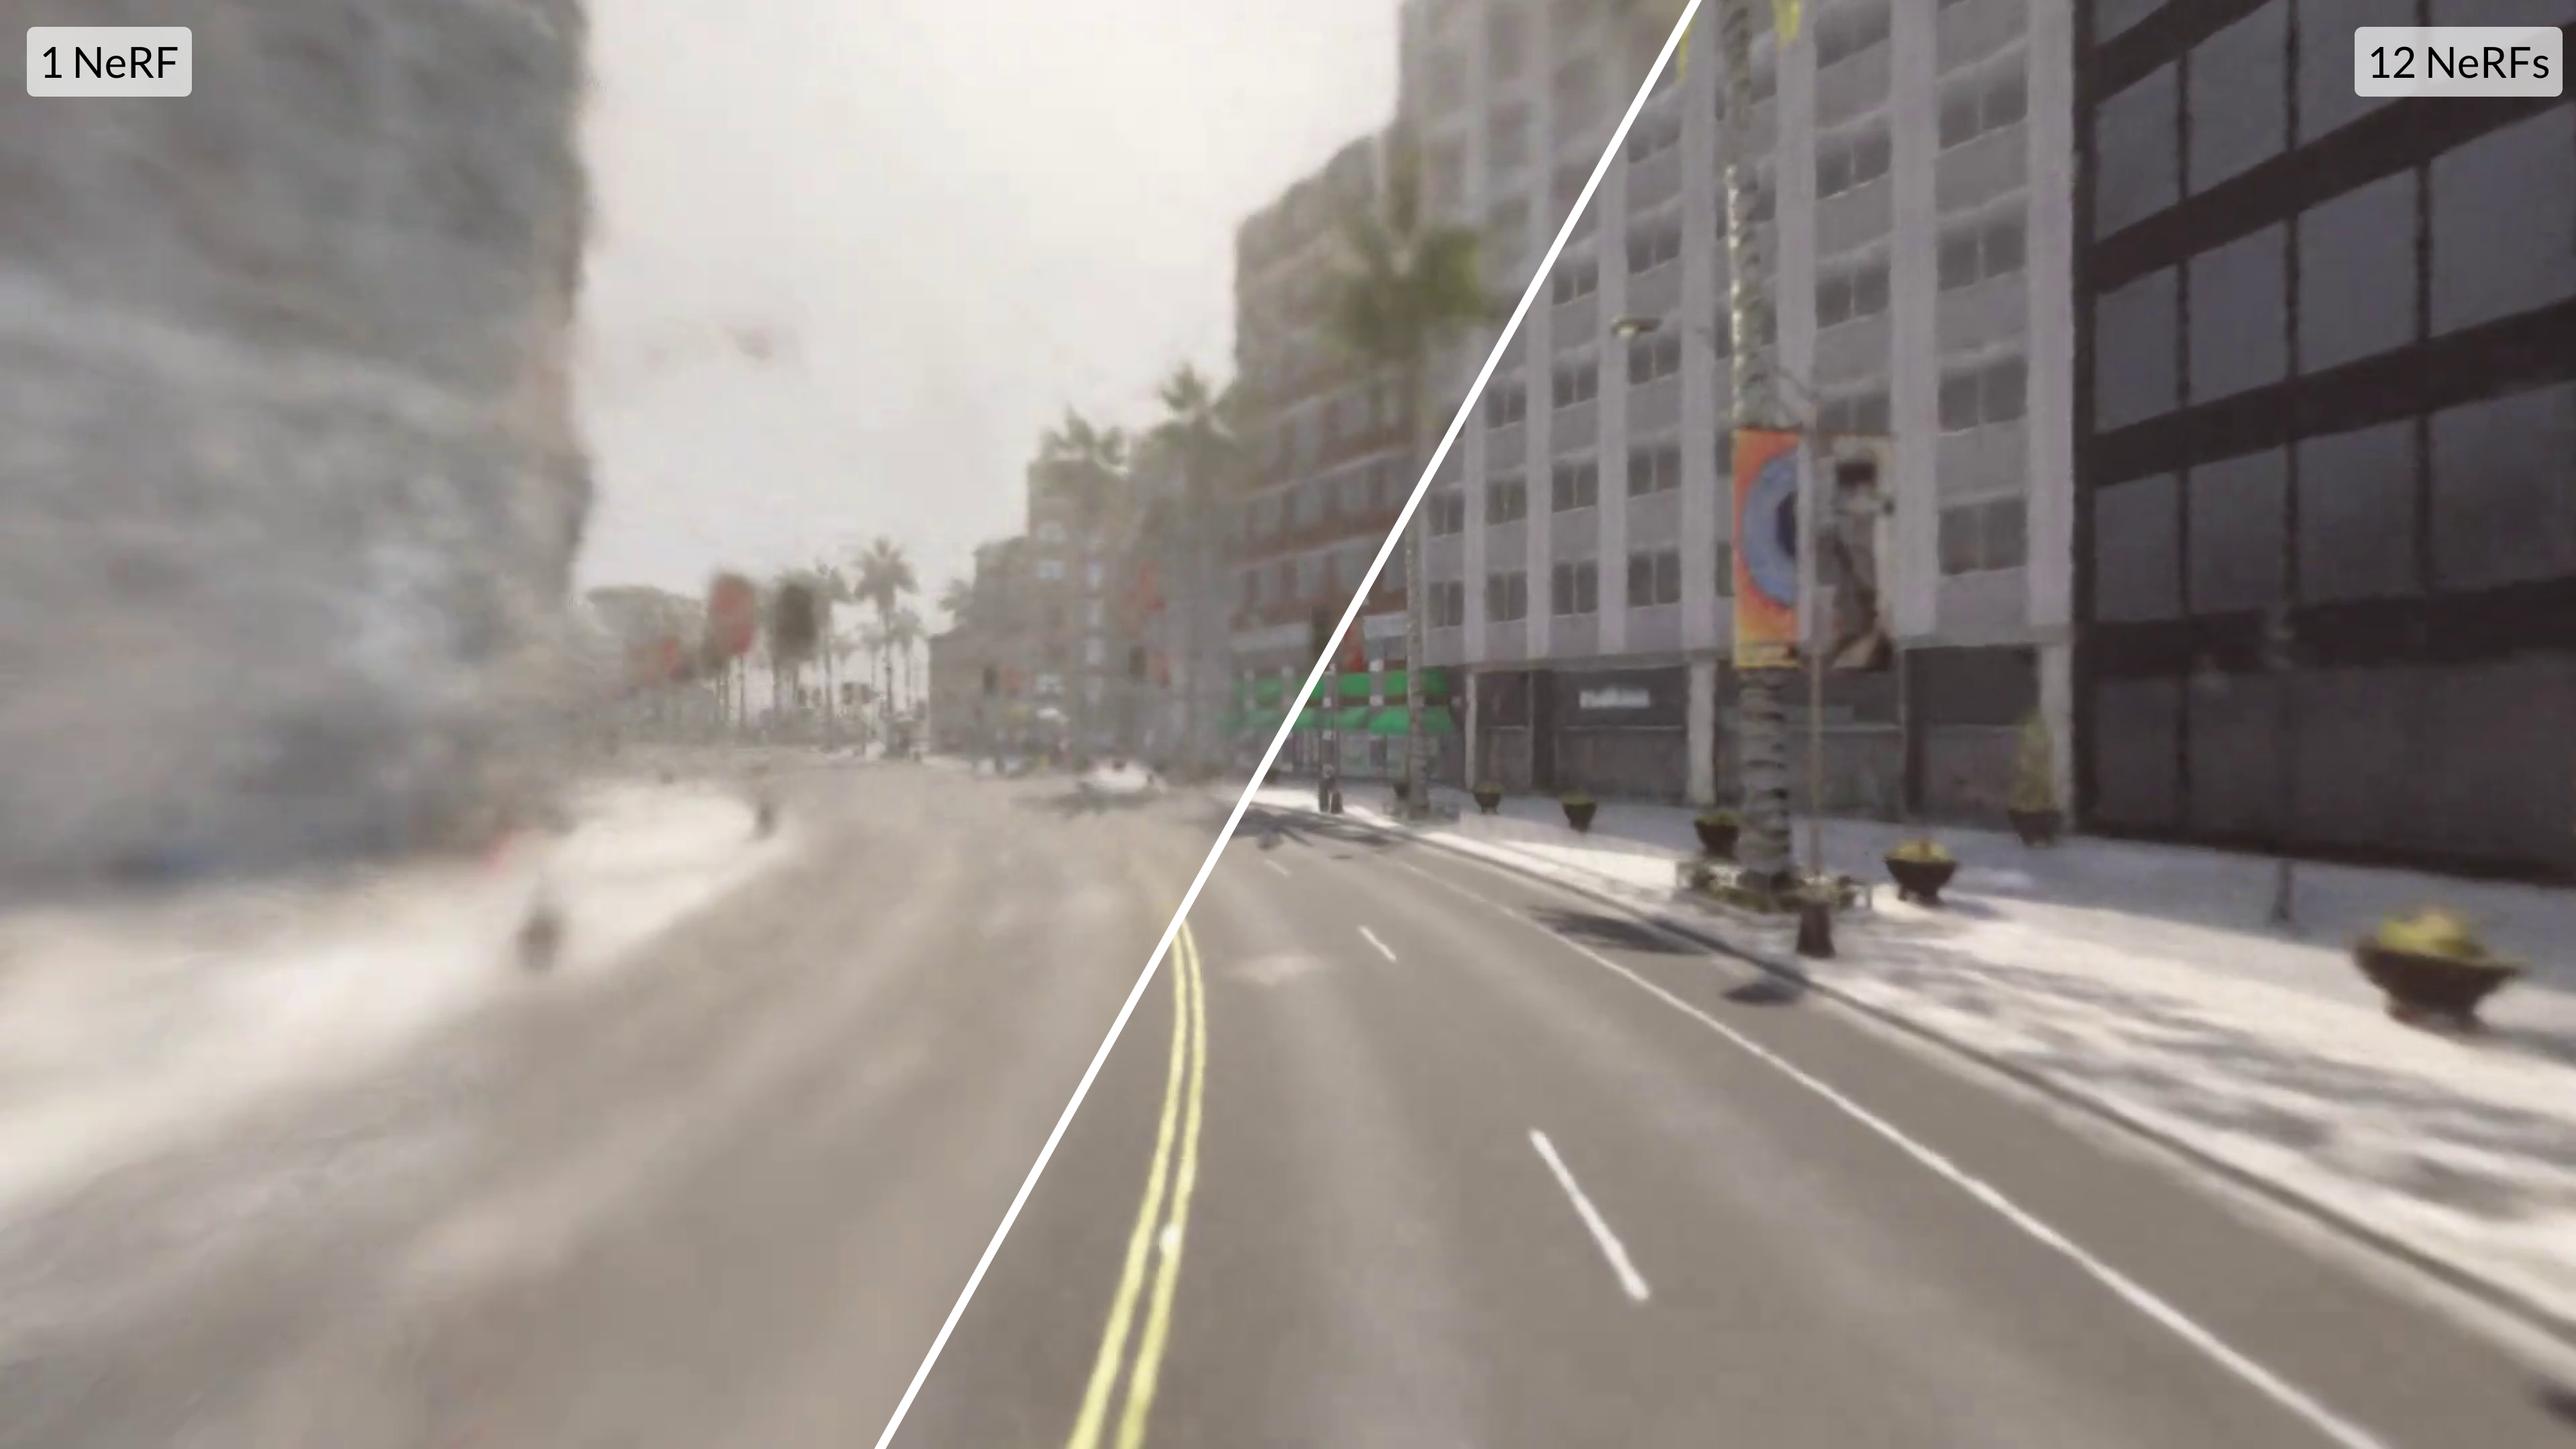
\includegraphics[width=1.0\textwidth]{figures/block-nerf-comparison.png}
    \caption{Comparison of two renders from models who have been trained on the same data. Left) One NeRF trained on all data, Right) 12 NeRFs trained on equally spaced segments.}
    \label{fig:block-nerf-comparison}
\end{figure}

Our experimental results demonstrate that Block NeRF is capable of generating high-quality results for large scenes, where a single NeRF may start to deteriorate as the scene size increases. We show that by splitting the scene into smaller segments, the combined scene generates better results than when the entire scene is trained within a single NeRF. These findings suggest that Block NeRF is a promising approach for generating high-quality results for large-scale scenes.

\subsection{Improving Block NeRF}
As seen in the previous section, the naive Block NeRF implementation improves the capacity and subsequently quality of the image synthesis across large scenes. One of the issues with the naive implementation is the hard cutoff between each block where $\text{block}_i$ only trains on a single data-bin $[\text{data}_i, \text{data}_{i + 1}]$ where each data-bin $\text{data}_i$ is a disjunct collection of images and corresponding camera poses. This leads to blurry artifacts in the first frames of a new block, as can be seen in \autoref{fig:block-nerf-frame-comparison}.

\begin{figure}[!h]
    \centering
    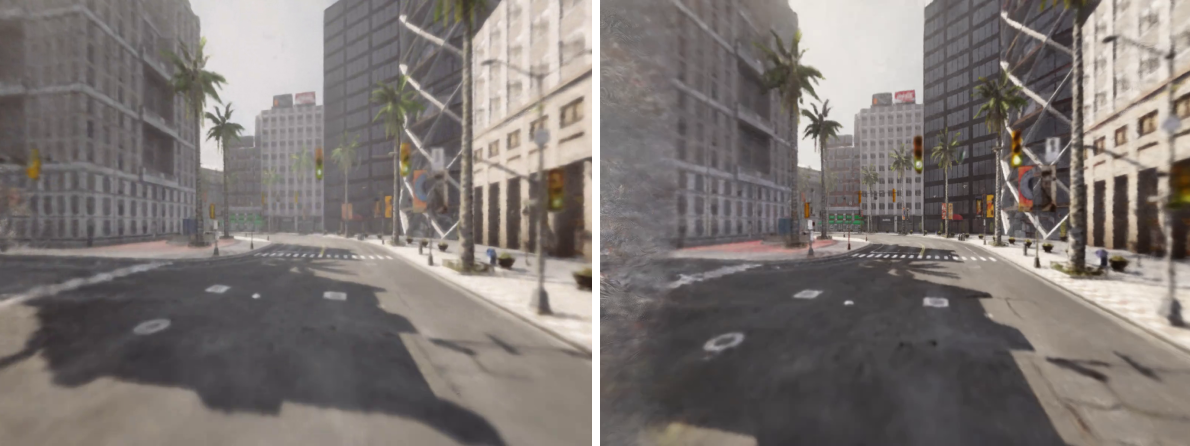
\includegraphics[width=1.0\textwidth]{figures/block-nerf-frame-comparison.png}
    \caption{Comparison of two consecutive frames of a single render on a 12 block NeRF. The first frame (left) is the last frame rendered by block number 1. The second frame (right) is the first frame rendered by block number 2. The details of the scenery in the second frame is clearly better than the first, which is expected as block number 2 have been trained on close-up images of the scene. This difference could be mitigated by looking into image merging techniques such as inverse distance weighing.}
    \label{fig:block-nerf-frame-comparison}
\end{figure}

In order to remedy these artifacts, the data-bins can be expanded to contain an overlap of the data from the previous and successive data-bin. $\text{Block}_i$ would, in the general case where it's not the first or last index of the data-bin array, train on data $[\text{data}_i + \text{data}_{i-1}[overlap:], \text{data}_{i + 1} + \text{data}_{i+2}[:overlap]]$. A qualitative comparison of the effects from this can be seen in \autoref{fig:overlap}.

\begin{figure}[ht]
    \centering
    \includegraphics[width=1.0\textwidth]{figures/overlap.png}
    \caption{Comparison of Block-NeRF trained with 0, 50 and 100 images overlap, respectively.}
    \label{fig:overlap}
\end{figure}

\begin{table}[ht]
\centering
\setlength{\tabcolsep}{6pt}
\renewcommand{\arraystretch}{1.5}
\begin{tabular}{l | C{2.2} C{1.3} C{1.3}}
\hline
\textbf{Description} & \textbf{PSNR $\uparrow$} & \textbf{SSIM $\uparrow$} & \textbf{LPIPS $\downarrow$} \\
\hline
Average 100 overlap &\cellcolor{red}23.7983296667 &\cellcolor{red}0.7459294167 &\cellcolor{red}0.24848525 \\
Average 50 overlap & 24.3081965833 & 0.7760105833 & 0.2063403333 \\
Average 0 overlap &\cellcolor{green}24.7952365 &\cellcolor{green}0.8017453333 &\cellcolor{green}0.157845 \\
\hline
\end{tabular}
\caption{Average across different Block NeRF overlap configurations. The overlap becomes less visible with higher overlap values, but it comes at the cost of the previously explored capacity issue.}
\label{tab:block-nerf-overlap-comparison}
\end{table}


\begin{comment}
\begin{table}
\centering
\begin{tabular}{|l|c|c|c|c|}
\toprule
& description & psnr & ssim & lpips \\
\midrule
0 & 0 & 24.022085 & 0.785746 & {\cellcolor{red}} 0.188386 \\
1 & 1 & 23.930248 & 0.758505 & 0.244230 \\
2 & 2 & 23.802164 & 0.744722 & 0.260637 \\
3 & 3 & 23.783644 & 0.751682 & 0.217054 \\
4 & 4 & {\cellcolor{green}} 24.798885 & {\cellcolor{green}} 0.788536 & 0.224305 \\
5 & 5 & 23.982912 & 0.774523 & 0.243821 \\
6 & 6 & 24.080154 & 0.738190 & 0.269370 \\
7 & 7 & 23.214962 & 0.714268 & 0.276262 \\
8 & 8 & 23.937700 & 0.756132 & 0.229545 \\
9 & 9 & 23.565117 & 0.710089 & 0.283474 \\
10 & 10 & {\cellcolor{red}} 22.669729 & {\cellcolor{red}} 0.679423 & {\cellcolor{green}} 0.304618 \\
11 & 11 & 23.792356 & 0.749337 & 0.240121 \\
\hline
\multicolumn{2}{l}{Average} & 23.7983296667 & 0.7459294167 & 0.24848525 \\
\hline
\end{tabular}
\caption{Results for exp\_block\_nerf\_long\_path\_2\_overlap\_100-block\_10}
\label{tab:exp_block_nerf_long_path_2_overlap_100-block_10}
\end{table}

\begin{table}
\centering
\begin{tabular}{|l|c|c|c|c|}
\toprule
& description & psnr & ssim & lpips \\
\midrule
0 & 0 & 24.699778 & 0.810479 & {\cellcolor{red}} 0.164481 \\
1 & 1 & 24.626417 & 0.787247 & 0.201674 \\
2 & 2 & 24.641893 & 0.794024 & 0.209372 \\
3 & 3 & {\cellcolor{red}} 23.378580 & 0.734546 & 0.212338 \\
4 & 4 & {\cellcolor{green}} 25.154751 & {\cellcolor{green}} 0.813535 & 0.189947 \\
5 & 5 & 24.988750 & 0.808827 & 0.200096 \\
6 & 6 & 24.227613 & 0.780267 & 0.219571 \\
7 & 7 & 23.810534 & 0.741920 & 0.215074 \\
8 & 8 & 24.395237 & 0.784949 & 0.197768 \\
9 & 9 & 23.838959 & 0.738407 & 0.237455 \\
10 & 10 & 23.702843 & {\cellcolor{red}} 0.729783 & {\cellcolor{green}} 0.237854 \\
11 & 11 & 24.233004 & 0.788143 & 0.190454 \\
\hline
\multicolumn{2}{l}{Average} & 24.3081965833 & 0.7760105833 & 0.2063403333 \\
\hline
\end{tabular}
\caption{Results for exp\_block\_nerf\_long\_path\_2\_overlap\_50-block\_10}
\label{tab:exp_block_nerf_long_path_2_overlap_50-block_10}
\end{table}

\begin{table}
\centering
\begin{tabular}{|l|c|c|c|c|}
\toprule
& description & psnr & ssim & lpips \\
\midrule
0 & 0 & 24.987898 & 0.825968 & 0.134750 \\
1 & 1 & 25.734240 & 0.830594 & 0.151921 \\
2 & 2 & 24.752632 & 0.833735 & 0.145856 \\
3 & 3 & {\cellcolor{red}} 22.755438 & {\cellcolor{red}} 0.715347 & {\cellcolor{green}} 0.201178 \\
4 & 4 & 25.325920 & 0.837257 & {\cellcolor{red}} 0.133863 \\
5 & 5 & 25.745651 & {\cellcolor{green}} 0.841267 & 0.143897 \\
6 & 6 & {\cellcolor{green}} 25.748047 & 0.823805 & 0.161235 \\
7 & 7 & 25.158396 & 0.771797 & 0.156722 \\
8 & 8 & 25.061327 & 0.816051 & 0.151580 \\
9 & 9 & 23.696585 & 0.756446 & 0.185149 \\
10 & 10 & 24.036982 & 0.759052 & 0.186791 \\
11 & 11 & 24.539722 & 0.809625 & 0.141198 \\
\hline
\multicolumn{2}{l}{Average} & 24.7952365 & 0.8017453333 & 0.157845 \\
\hline
\end{tabular}
\caption{Results for exp\_block\_nerf\_long\_path\_2\_REDONE\_2-block\_10}
\label{tab:exp_block_nerf_long_path_2_REDONE_2-block_10}
\end{table}
\end{comment}



\begin{comment}
\begin{table}[ht]
\centering
\setlength{\tabcolsep}{6pt}
\renewcommand{\arraystretch}{1.5}
\begin{tabular}{l l | C{2.2} C{1.3} C{1.3}}
\hline
& \textbf{Description} & \textbf{PSNR $\uparrow$} & \textbf{SSIM $\uparrow$} & \textbf{LPIPS $\downarrow$} \\
\hline
0 & 0 & \cellcolor{red} 22.515461 & \cellcolor{red} 0.654036 & \cellcolor{red} 0.424356 \\
1 & Average of 12 block NeRF & \cellcolor{green} 24.774259 & \cellcolor{green} 0.801090 & \cellcolor{green} 0.159331 \\
\hline
\end{tabular}
\caption{Results for exp\_block\_nerf\_long\_path\_no\_blocks-0 compared to the results of exp\_block\_nerf\_long\_path\_2-block\_10}
\label{tab:exp_block_nerf_long_path_no_blocks-0}
\end{table}
\end{comment}